\documentclass[aps,prx,reprint,superscriptaddress,floatfix]{revtex4-2}

\usepackage[T1]{fontenc}
\usepackage{amsmath,amssymb,amsfonts,amsthm,bm}
\usepackage{booktabs,array,multirow}
\usepackage{graphicx}
\usepackage{microtype}
\usepackage[colorlinks=true,allcolors=blue]{hyperref}
\usepackage{url}

\newtheorem{theorem}{Theorem}[section]
\newtheorem{proposition}[theorem]{Proposition}
\newtheorem{lemma}[theorem]{Lemma}
\newtheorem{corollary}[theorem]{Corollary}
\newtheorem{assumption}[theorem]{Assumption}
\newcommand{\E}{\mathbb{E}}
\newcommand{\Pp}{\mathbb{P}}
\newcommand{\R}{\mathbb{R}}
\newcommand{\AURC}{\mathrm{AURC}}
\newcommand{\argminop}{\operatorname*{arg\,min}}
\newcommand{\ConfirmN}{160}
\newcommand{\ConfirmGlobalAURC}{0.17277}
\newcommand{\ConfirmGatedAURC}{0.16930}
\newcommand{\ConfirmFamilyAURC}{0.17207}
\newcommand{\ConfirmOracleAURC}{0.16048}
\newcommand{\ConfirmDelta}{-0.002768}
\newcommand{\ConfirmCILow}{-0.005696}
\newcommand{\ConfirmCIHigh}{-0.00008178}
\newcommand{\ConfirmAccepted}{12}
\newcommand{\ConfirmHarms}{4}
\newcommand{\ConfirmJointHarmRate}{0.0250}
\newcommand{\ConfirmConditionalHarmRate}{0.333}
\newcommand{\ConfirmCoverage}{0.88125}
\newcommand{\ConfirmNominal}{0.90}
\newcommand{\ConfirmAcceptedRate}{0.075}
\newcommand{\ConfirmOpportunity}{0.071}
\newcommand{\ConfirmBAdelta}{+0.003764}
\newcommand{\ConfirmRRdelta}{-0.013269}
\newcommand{\ConfirmWSdelta}{-0.001567}
\newcommand{\DevDelta}{-0.009370}
\newcommand{\DevCILow}{-0.016454}
\newcommand{\DevCIHigh}{-0.002500}
\newcommand{\DevAccepted}{10}
\newcommand{\DevHarms}{1}
\newcommand{\DevCoverage}{0.9375}
\newcommand{\ProtocolHash}{58692d57df9cb489ab22fa0cc672924d5b3888d107aee0a88b856c726ac5dcf1}
\newcommand{\DecisionHash}{962f63d71dc20efa5896a949a2d4869bb1c691395b65ecb1d079302e4805bbe6}
\newcommand{\ImplementationHash}{42aa34816315126b4519d92da86a24120443cdee6a654cf92c932c7b91ce9f3d}
\newcommand{\ConfigHash}{a0e66aa4c41f7868dd0a4ae1ca1223de7a1d92caebf7857062f033261f56d558}


\hypersetup{
  pdftitle={Query-Efficient Quantum Approximate Optimization via Graph-Conditioned Trust Regions},
  pdfauthor={Molena Huynh},
  pdfsubject={Fixed-budget optimizer portfolios and reliability auditing},
  pdfkeywords={QAOA, trust regions, algorithm selection, selective prediction, reproducibility}
}

\begin{document}

\title{Query-Efficient Quantum Approximate Optimization
via Graph-Conditioned Trust Regions}
\author{Molena Huynh}
\email{molena.huynh@jmp.com}
\affiliation{North Carolina State University, Raleigh, North Carolina 27695, USA}
\date{July 2026}

\begin{abstract}
Classical optimization can dominate the measurement cost of a variational
quantum algorithm, yet learned optimizer routing may be less reliable than a
fixed schedule.  We cast graph-conditioned trust regions as a target-free,
fixed-budget portfolio for depth-two MaxCut QAOA in which nine arms share a
$32$-call ceiling.  A ridge model predicts each arm's anytime regret, a known
graph family supplies a strong fallback, and a one-sided residual order
statistic abstains whenever the predicted improvement is not certified.  After a
$64$-graph development audit, the selector is fit on $48$ graphs, calibrated on
$48$ disjoint graphs, and locked before a single evaluation on $160$ instances.
Gated deployment attains mean regret $\ConfirmGatedAURC$ against
$\ConfirmFamilyAURC$ for the fallback, but accepts only $\ConfirmAccepted$
routes, four of them harmful.  One-sided empirical coverage is
$\ConfirmCoverage$, below the frozen $\ConfirmNominal$ requirement, so the
reliability claim fails; fixed family quotas also preclude a pooled
exchangeability certificate.  The contribution is a reproducible
exact-statevector failure analysis, not evidence of hardware, scaling, or
quantum advantage.
\end{abstract}
\keywords{quantum approximate optimization, algorithm selection, trust regions,
selective prediction, fixed-budget optimization, reproducibility}
\maketitle

\section{Introduction}

A variational quantum algorithm pairs a parameterized circuit with a classical
optimizer \citep{peruzzo2014variational,mcclean2016theory}.  Its near-term
appeal comes with a stubborn cost problem: each black-box objective query can
demand many circuit preparations and measurements
\citep{preskill2018quantum,bharti2022noisy}, so the optimizer belongs to the
physical resource model rather than to interchangeable software
\citep{cerezo2021variational}.

The quantum approximate optimization algorithm (QAOA) makes the coupling
concrete by alternating cost and mixer unitaries before optimizing a small angle
vector \citep{farhi2014qaoa,hadfield2019alternating}, with combinatorial
objectives encoded as Ising Hamiltonians \citep{lucas2014ising}.  Its empirical
behavior turns on graph structure, depth, initialization, and search budget
\citep{zhou2020qaoa}.  Angle concentration can make fixed schedules competitive
on typical instances \citep{brandao2018fixed,akshay2021concentration}, warm
starts can inject classical solutions \citep{egger2021warm}, and transferred
parameters can exploit similarity across weighted graphs
\citep{shaydulin2023weighted}.

Graph-conditioned optimization tries to use this shared structure before or
during search: a predictor can propose angles, a local covariance, a trust
region, or an optimizer choice.  Learned graph initializers demonstrate the
opportunity \citep{jain2022gnn}, and learned variational optimizers show that
trajectories themselves can be predicted \citep{khairy2020learning}.  The
statistical question is rarely stated: when should a learned recommendation
displace a strong, cheap control?

That question cannot be settled by average terminal quality.  Tuning and
selection on the same benchmark used for evaluation introduce substantial
optimism \citep{cawley2010overfitting}, a router can raise a pooled mean by
helping one family while harming another, and a target-based stopping rule can
depend on an oracle unavailable in deployment.  The classical algorithm-selection
problem already separates instance features, candidate algorithms, and
performance measures \citep{rice1976selection}; the quantum setting merely adds
an unusually expensive response surface.

We therefore replace privileged target hitting with a fixed-query anytime
metric.  Every arm receives $32$ objective calls, and utility is the average
normalized regret over the checkpoints $\{1,2,4,8,16,32\}$.  A
relabeling-invariant structural model predicts each arm's utility, the strongest
development arm within the known graph family is the fallback, and routing is
accepted only when an upper residual order statistic indicates that the selected
arm should beat that fallback.  The abstention rule borrows split-conformal
reasoning \citep{vovk2005algorithmic,angelopoulos2021gentle}, whose finite-sample
guarantee needs exchangeability; because our confirmatory design uses fixed
family quotas with sequential non-isomorphism filtering, we report the frozen
rule together with the limits of its coverage interpretation
\citep{barber2022exchangeability}.

Figure~\ref{fig:protocol} fixes the evidence chronology.  Development fits the
selector and family fallback, calibration fixes one residual order statistic, the
graph list, code, configuration, and decision are hashed, and the audit is
evaluated once.  This chronology matters as much as the model, because
unrecorded iteration on audit outcomes would erase the meaning of a confirmatory
result.  The final decision is negative: the deployed policy slightly improves
mean anytime regret, accepts only $\ConfirmAccepted$ of $\ConfirmN$ routes,
harms four accepted instances, and misses the frozen coverage threshold.  A
favorable mean coexisting with a failed reliability criterion is the distinction
this paper is built to preserve.

\begin{figure*}[tbp]
\centering
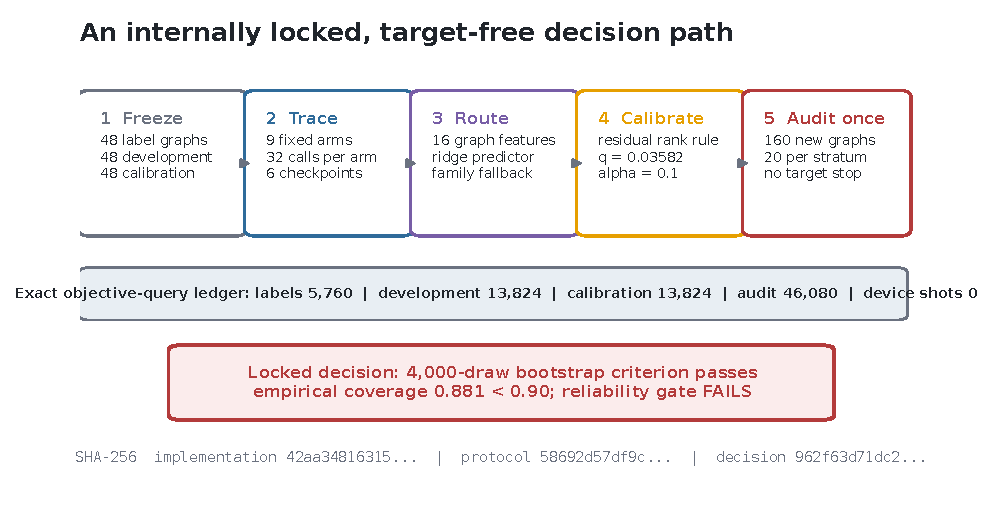
\includegraphics[width=0.98\textwidth]{figures/Figure1_PortfolioProtocol.pdf}
\caption{\textbf{Internally locked fixed-budget protocol.}  Development data fit
the structural selector and family fallback; calibration fixes a one-sided
residual order statistic.  The graph list, implementation, configuration, and
decision are hashed before the $\ConfirmN$-graph audit is evaluated.}
\label{fig:protocol}
\end{figure*}

\section{Background}

\subsection{Quantum Approximate Optimization}

For an unweighted graph $G=(V,E)$, define
\begin{equation}
 C_G=\sum_{(u,v)\in E}\frac{I-Z_uZ_v}{2},
 \qquad B=\sum_{v\in V}X_v .
 \label{eq:operators}
\end{equation}
A depth-$p$ QAOA state is
\begin{equation}
 |\bm\gamma,\bm\beta\rangle =
 \prod_{j=p}^{1}e^{-i\beta_jB}e^{-i\gamma_jC_G}
 |+\rangle^{\otimes |V|},
 \label{eq:qaoa}
\end{equation}
with objective
$F_G(\bm\theta)=\langle\bm\gamma,\bm\beta|C_G|\bm\gamma,\bm\beta\rangle$.
Analytic parameter-shift rules evaluate gradients on compatible hardware
\citep{schuld2019evaluating,wierichs2022general}, whereas stochastic estimators
trade coordinate resolution for fewer objective calls \citep{spall1992spsa}.

Gradient methods do not dissolve trainability concerns.  Random or highly
expressive circuits can exhibit barren plateaus \citep{mcclean2018barren};
expressibility is tied to gradient concentration \citep{holmes2022connecting};
and control-theoretic tools sharpen the diagnosis
\citep{larocca2022diagnosing}.  Gradient-free search likewise degrades in flat
landscapes \citep{arrasmith2021effect}.  We therefore compare complete
fixed-budget trajectories instead of presuming one access model is uniformly
best.

\subsection{Fixed-Budget Black-Box Optimization}

At the checkpoints $\mathcal T=\{1,2,4,8,16,32\}$, arm $a$ on instance $i$ has
post hoc normalized regret
\begin{equation}
 r_{ia}(t)=1-
 \frac{\max_{s\le t}F_{G_i}(\bm\theta_{ias})}{C_{\max}(G_i)}
 \label{eq:regret}
\end{equation}
and utility
\begin{equation}
 u_{ia}=\AURC_{ia}=
 \frac{1}{|\mathcal T|}\sum_{t\in\mathcal T}r_{ia}(t),
 \label{eq:aurc}
\end{equation}
where lower is better.  Exact MaxCut $C_{\max}$ enters only after optimization;
no arm ever observes a target or a target-hitting event.

The portfolio spans fixed schedules, transferred angles, multistart, SPSA, and
the graph-conditioned trust-region arm, a heterogeneity that reflects the fact
that optimizer rankings depend on the problem and budget
\citep{bonet2023performance}.  Mesh-adaptive direct search gives a principled
derivative-free comparator \citep{audet2006mesh}, BOBYQA maintains a bounded
quadratic model \citep{powell2009bobyqa}, and covariance-matrix adaptation learns
a search distribution \citep{hansen2001cma}.  We keep the simpler arms because a
portfolio is only meaningful relative to its actual controls, and a ramped
fixed schedule is a strong low-complexity baseline \citep{montanez2025ramp}.

\subsection{Selective Routing and Risk}

Let $x(G)\in\R^{16}$ be a relabeling-invariant graph summary and
$\widehat u_a(x)$ the predicted utility of arm $a$.  The proposed arm is
\begin{equation}
 s(x)=\argminop_a\widehat u_a(x).
 \label{eq:selected}
\end{equation}
For family label $f$, the fallback $b(f)$ is the development arm of minimum
family-mean utility.  Define the realized selected-minus-fallback regret and its
prediction residual
\begin{equation}
 \Delta=u_s-u_b,
 \qquad
 R=\Delta-(\widehat u_s-\widehat u_b).
 \label{eq:residual}
\end{equation}
Given a calibration upper order statistic $q$, routing is accepted when
\begin{equation}
 \widehat u_s-\widehat u_b+q<0,
 \label{eq:gate}
\end{equation}
and otherwise abstains to $b(f)$.  This is selective prediction, in which
coverage, acceptance, joint harm, and conditional harm are different quantities.
Conformalized quantile regression can adapt interval width to covariates
\citep{romano2019cqr}, and exact binomial limits can summarize observed event
rates \citep{clopper1934fiducial}, but neither licenses a coverage claim without
a sampling model.

\section{Related Work}

QAOA initialization exploits concentration, interpolation, and problem structure
\citep{zhou2020qaoa,brandao2018fixed}, and learned graph initializers extend the
idea through message passing \citep{jain2022gnn}.  Weighted-MaxCut parameter
transfer targets related objectives \citep{shaydulin2023weighted}, while ramp
schedules supply a strong low-complexity comparator \citep{montanez2025ramp}.
Our portfolio treats these ideas as arms or controls rather than assuming one
initialization dominates.

Graph convolutional networks use normalized neighborhood aggregation
\citep{kipf2017gcn}, graph attention learns neighbor weights
\citep{velickovic2018gat}, and graph-isomorphism networks characterize a powerful
message-passing class \citep{xu2019gin}.  We deliberately use $16$ hand-computed
invariant summaries with ridge regression; the low-capacity choice reduces model
flexibility and makes every routing score inspectable.

Bayesian optimization is another route to expensive black-box search.  Efficient
global optimization introduced improvement-based acquisition
\citep{jones1998efficient}, practical formulations popularized Gaussian-process
tuning \citep{snoek2012practical}, a broad review organized surrogate and
acquisition choices \citep{shahriari2016taking}, and differentiable Monte Carlo
acquisitions are available in modern toolkits \citep{balandat2020botorch}.  These
may be useful arms, yet fitting a surrogate does not make its objective
evaluations free.

Algorithm configuration learns settings across tasks: sequential model-based
configuration proposes new settings from prior runs \citep{hutter2011sequential},
and SMAC3 exposes a reproducible modern package \citep{lindauer2022smac3}.  The
portfolio view also touches active subspaces \citep{constantine2015active},
sliced inverse regression \citep{li1991sliced}, and regression graphics
\citep{cook1998regression}, though our predictor reduces neither the circuit
parameter dimension nor the feature dimension adaptively.  Randomized linear
algebra would matter for future low-rank structural models: randomized range
finding and blocked QB give scalable, adaptive-rank approximation
\citep{halko2011finding,yu2018randqb}, sketching offers streaming alternatives
\citep{woodruff2014sketching,liberty2013simple}, and matrix concentration
supplies probabilistic tools \citep{tropp2015matrix}; none is needed for the
released $16$-feature ridge fit.  Finally, statistical safeguards address
distinct risks: bootstrap resampling estimates sampling variation
\citep{efron1993bootstrap}, multiple-testing procedures control false discoveries
\citep{benjamini1995controlling}, the Neyman--Pearson framework separates size
from power \citep{neyman1933efficient}, and cross-data-set comparison must occur
at the data-set level \citep{demsar2006statistical}.

\section{Failure Modes of Structural Optimizer Routing}

\subsection{Selection Bias and Distribution Shift}

Choosing a route because it is best on development data is not a
distribution-free argument.  Even a perfect empirical ranking can invert under
task shift, a basic distinction in algorithm selection and honest model
assessment \citep{rice1976selection,cawley2010overfitting}.

\begin{theorem}[Near-maximal excess loss after routing shift]
\label{thm:shift}
For every $\varepsilon\in(0,1)$ there exist two optimizer arms $a,b$, losses in
$[0,1]$, a development distribution $P_0$, and a deployment distribution $P_1$
such that $a$ is the unique risk minimizer under $P_0$, $b$ is the unique risk
minimizer under $P_1$, and routing unconditionally to $a$ has deployment excess
risk $1-\varepsilon$.
\end{theorem}

Appendix~\ref{app:proof-shift} gives a complete construction.  The theorem is
elementary by design: no model complexity is required to produce a failure,
which is exactly why graph splits, family strata, and chronology must be declared
before a learned router is interpreted.  The project's first version optimized
against an offline target and compared a learned trust-region policy mainly with
random restart; stronger fixed schedules were cheaper, and the target was
unavailable at deployment.  The present portfolio keeps that history as a legacy
diagnostic and does not merge it with the target-free confirmatory result.

The one-shot outcome and its family concentration are displayed in
Fig.~\ref{fig:confirm}.

\begin{figure*}[tbp]
\centering
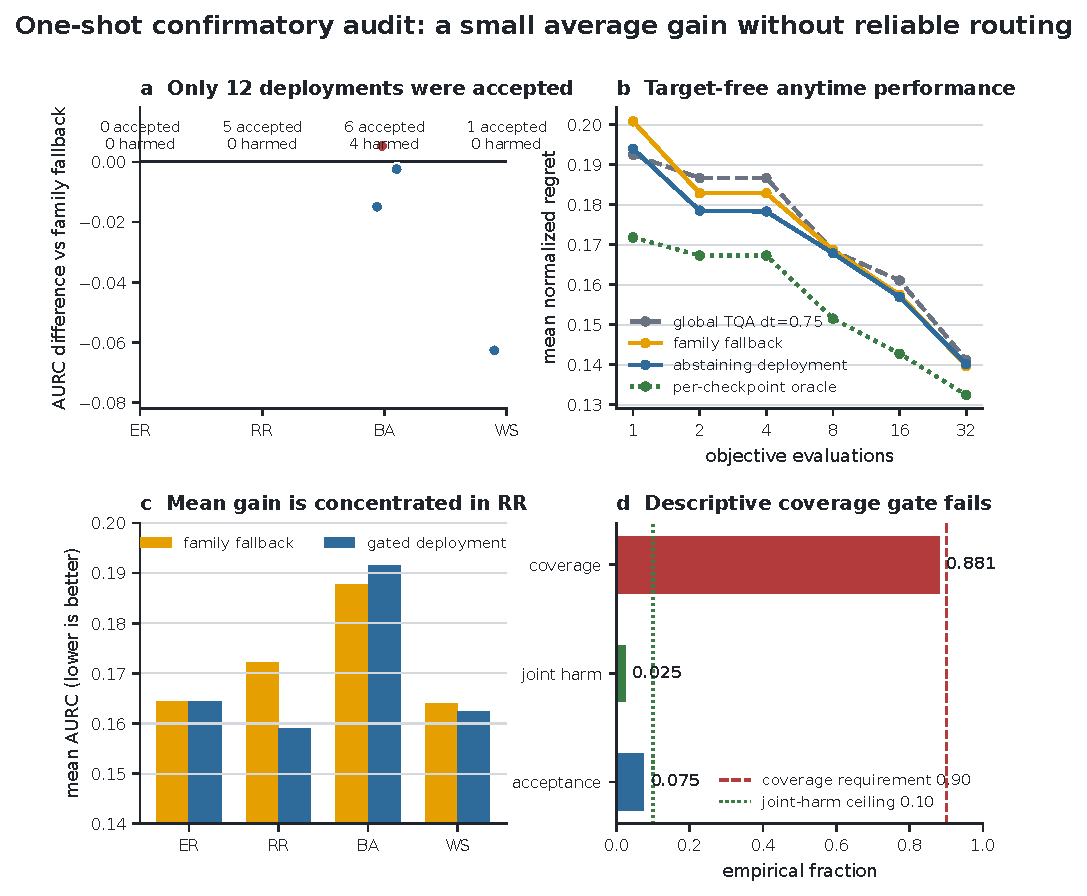
\includegraphics[width=0.98\textwidth]{figures/Figure2_ConfirmatoryAudit.pdf}
\caption{\textbf{One-shot confirmatory audit.}  The mean gain is small and
concentrated by family.  Twelve routes are accepted, four are harmful, and
descriptive one-sided coverage misses the frozen requirement.}
\label{fig:confirm}
\end{figure*}

\subsection{Coverage and Conditional Harm}

Let $A$ be the event that the selector accepts a route and $H=\{\Delta>0\}$ the
event that the selected arm is worse than the fallback.

\begin{proposition}[Harm-rate decomposition]
\label{prop:harm}
If $\Pp(A)>0$, then
\begin{equation}
 \Pp(A\cap H)=\Pp(A)\,\Pp(H\mid A),
 \label{eq:harm}
\end{equation}
so controlling joint harm alone does not control conditional harm when
acceptance can be small.
\end{proposition}

The proof and an explicit counterexample are in Appendix~\ref{app:proof-harm}.
In the audit, $\Pp_n(A)=\ConfirmAccepted/\ConfirmN=\ConfirmAcceptedRate$,
$\Pp_n(A\cap H)=\ConfirmHarms/\ConfirmN=\ConfirmJointHarmRate$, and
$\Pp_n(H\mid A)=\ConfirmHarms/\ConfirmAccepted=\ConfirmConditionalHarmRate$.  The
joint rate is small because acceptance is small, not because accepted routes are
uniformly safe.  Marginal coverage is also distinct from selective harm: an upper
residual bound can cover $\Delta$ while acceptance concentrates errors near the
decision boundary, and conversely a policy can have acceptable joint harm while
missing a nominal residual-coverage target.  All four quantities must be
reported, because marginal calibration and conditional selection answer different
questions \citep{vovk2005algorithmic,angelopoulos2021gentle}.

\subsection{Acceptance, Exceedance, and Non-Certification}

Write $\widehat d=\widehat u_s-\widehat u_b$, $R=\Delta-\widehat d$,
$A=\{\widehat d+q<0\}$, and $H=\{\Delta>0\}$.  The acceptance rule has a
deterministic implication that needs no sampling model.

\begin{proposition}[Acceptance--exceedance containment]
\label{prop:containment}
For every joint distribution of $(\Delta,\widehat d)$ and every $q\in\R$,
\begin{equation}
 A\cap H\subseteq\{R>q\}.
 \label{eq:containment}
\end{equation}
Consequently, for any $\alpha\in[0,1]$, if $\Pp(R\le q)\ge1-\alpha$ then
$\Pp(A\cap H)\le\alpha$; if additionally $\Pp(A)>0$ then
$\Pp(H\mid A)\le\alpha/\Pp(A)$.
\end{proposition}

Appendix~\ref{app:proof-containment} proves every implication.  The result
clarifies both the appeal and the limit of residual calibration: idealized
marginal residual coverage controls joint harm, whereas the conditional bound
deteriorates as acceptance becomes rare.  More importantly, the locked
fixed-quota, sequentially filtered audit does not establish the pooled
exchangeability needed to infer the premise from the order statistic, so
Proposition~\ref{prop:containment} is an algebraic reading of the gate rather
than a certificate for the released audit \citep{barber2022exchangeability}.
Balancing an audit across families changes the sampling law: even if the final
order is randomized, family labels are dependent once their totals are fixed, so
comparisons must respect the stratum as the sampling unit
\citep{demsar2006statistical,efron1993bootstrap}.

\begin{proposition}[Fixed quotas are not pooled iid sampling]
\label{prop:quota}
Consider an audit of size $n$ with exactly $n_f$ graphs from family $f$, where
$0<n_f<n$, and let the order of the $n$ graphs be uniformly randomized.  For
distinct positions $i\ne j$, with
$Z_i=\mathbf 1\{\text{position }i\text{ has family }f\}$ and $p_f=n_f/n$,
\begin{equation}
 \operatorname{Cov}(Z_i,Z_j)=-\frac{p_f(1-p_f)}{n-1}<0.
 \label{eq:quota-covariance}
\end{equation}
Hence the pooled family labels are exchangeable but not independent, and the
audit is not an iid sample from the mixture with family mass $p_f$.
\end{proposition}

Appendix~\ref{app:proof-quota} proves the covariance identity by direct counting.
The proposition does not invalidate stratum-specific description or a
design-based analysis; it limits only an iid interpretation that ignores the
fixed quotas and sequential filtering.

Figure~\ref{fig:progression} contrasts the frozen development and confirmatory
decisions without reusing the audit split for tuning.

\begin{figure*}[tbp]
\centering
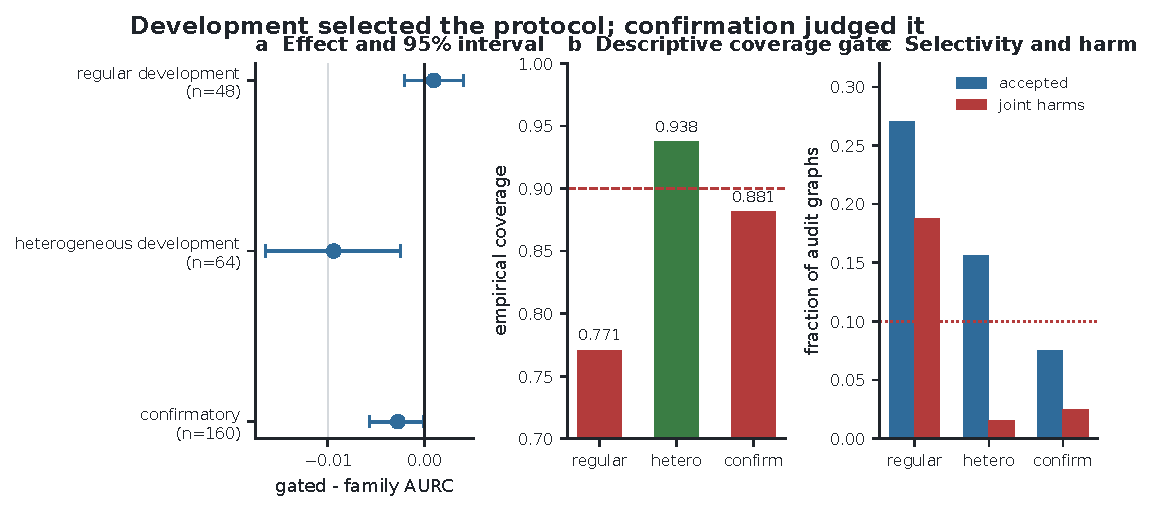
\includegraphics[width=0.98\textwidth]{figures/Figure3_DevelopmentToConfirmation.pdf}
\caption{\textbf{Development-to-confirmation progression.}  The heterogeneous
development split satisfies the frozen gate, while the confirmatory split misses
its empirical-coverage component.  Audit outcomes were not used to retune the
released decision.}
\label{fig:progression}
\end{figure*}

\section{Risk-Controlled Graph-Conditioned Trust Regions}

\subsection{Target-Free Portfolio Utility}

Every arm receives the same $32$-call counter; seed evaluations, restarts, and
all intermediate queries count against the ceiling.  The utility in
Eq.~\eqref{eq:aurc} rewards useful values early without granting any optimizer
access to $C_{\max}$, so the metric is target free for control even though exact
MaxCut remains a small-instance analysis oracle.  The nine arms are a
training-set concentration vector, four midpoint linear schedules,
one-nearest-neighbor transfer, four-start random multistart, SPSA, and the legacy
graph-conditioned Gaussian trust-region policy.  A fixed schedule can be
competitive because QAOA angles concentrate \citep{akshay2021concentration}, so
the portfolio retains simple arms instead of comparing only learned policies.

\subsection{Structural Prediction and Family Fallback}

The structural vector contains size, edges per vertex, density, seven degree
summaries, mean clustering, transitivity, triangles per vertex, and three
normalized-Laplacian summaries.  A multi-output ridge model predicts each arm's
utility,
\begin{equation}
 \widehat{\bm u}(x)=\bm a+W\widetilde x,
 \qquad \lambda_{\rm ridge}=1,
 \label{eq:ridge}
\end{equation}
where normalization uses development means and scales only.  The known synthetic
family label defines a strong deployable fallback, a choice deliberately
favorable to the control: the router must improve on what can be selected without
instance-level prediction.  General algorithm-selection theory warns that larger
portfolios raise both opportunity and overfitting risk
\citep{rice1976selection,cawley2010overfitting}.

\subsection{Residual Order-Statistic Abstention}

Fix $\alpha\in(0,1)$, and suppose calibration residuals $R_1,\dots,R_n$ and a
future residual $R_{n+1}$ are exchangeable and almost surely distinct.  Let
$k=\lceil(n+1)(1-\alpha)\rceil$ and let $q$ be the $k$th calibration order
statistic, with $q=+\infty$ when $k>n$.

\begin{theorem}[Split order-statistic coverage]
\label{thm:order}
Under these assumptions,
\begin{equation}
 \Pp(R_{n+1}\le q)=\frac{k}{n+1}\ge1-\alpha.
 \label{eq:coverage}
\end{equation}
\end{theorem}

Appendix~\ref{app:proof-order} proves the result by rank symmetry.  Ties are
handled conservatively or by randomized ranks.  The theorem explains the
calibration rule but does not assert that the quota-filtered audit residual is
exchangeable with the pooled calibration residuals; here $n=48$ and
$\alpha=0.10$ give the rank-$45$ upper statistic.

\subsection{Locked Confirmatory Decision}

The configuration, graph identities, angle labels, implementation, non-audit
traces, learned state, calibration statistic, and decision are hashed before the
audit is evaluated, and the evidence directory refuses a second audit run; the
generator revalidates these hashes before producing manuscript displays.  This
scheme is not an external preregistration and does not remove every researcher
degree of freedom.  The hashes establish internal consistency with the declared
execution order and the output lock refuses an overwrite, but they are not an
independent timestamp and cannot exclude unrecorded alternative runs.
Reproducibility here concerns both computational determinism and inferential
chronology.

\section{Experiments}

The locked benchmark asks whether a graph-conditioned selector lowers
fixed-budget anytime regret relative to a strong graph-family fallback and,
separately, whether accepted routes satisfy the declared reliability gate.
The population is a controlled Cartesian design over Erd\H{o}s--R\'enyi,
random-regular, Barab\'asi--Albert, and Watts--Strogatz generators with
$n\in\{12,14\}$ and QAOA depth two.  Graph identities separate 48 angle-label
instances, 48 development instances, 48 calibration instances, and 160
untouched audit instances.  The graph is the statistical sampling unit; family
and size define the eight fixed bootstrap strata.

Nine frozen optimizer arms receive the same 32 exact-objective-call ceiling:
concentration, four transferred fixed schedules, nearest-neighbor transfer,
random multistart, SPSA, and legacy GCTR.  Development fixes the ridge router
and family fallback, calibration fixes the one-sided residual order statistic,
and the audit is scored once without refitting.  The primary endpoint is
selected-minus-family-fallback area under the normalized anytime-regret curve;
secondary endpoints are acceptance, empirical one-sided coverage, joint and
conditional harm, family effects, and the complete offline/deployment resource
ledger.  The interval is a frozen 4,000-resample percentile bootstrap within
family-size strata, while the conjunctive go/no-go rule also requires portfolio
opportunity, negative interval endpoints, at least ten accepted graphs,
coverage at least 0.90, and joint harm at most 0.10.  The simulator uses exact
complex-128 statevectors: there are no shots, device noise, compilation, queue
latency, or hardware claims.  Runs use Python 3.13.12, NumPy 2.4.3, SciPy
1.17.1, NetworkX 3.6.1, PyTorch 2.11.0, Matplotlib 3.10.8, and pandas 3.0.2
on CPU, with master seed 20260719.  From the repository root,
\texttt{python run.py release} regenerates validated displays, checks source
synchronization and evidence hashes, builds the manuscript and source archive,
and fails on drift; \texttt{gctr-reproduce-all replay} and its
\texttt{full --quick} mode provide installed-package replay and reduced-cost
execution.

\subsection{Development Selection}

Graphs come from four synthetic families: Erd\H{o}s--R\'enyi
\citep{erdos1959random}, random regular as generated by NetworkX
\citep{hagberg2008networkx}, Barab\'asi--Albert \citep{barabasi1999emergence},
and Watts--Strogatz \citep{watts1998collective}.  Sequential filtering rejects
isomorphic repeats within each stratum, and separate angle-label, development,
calibration, and audit splits are frozen by graph identity.  An initial
fixed-parameter generator grid used all four families without broad parameter
variation; a subsequent $64$-graph heterogeneous development audit used declared
ranges and triggered the family-fallback protocol.  The locked selector was then
fit on $48$ development graphs and its residual threshold computed from $48$
disjoint calibration graphs, all before the confirmatory list and decision were
frozen.

For any split of $N$ graphs, let $\bar u_{\rm global}$ be the mean utility of the
single global arm and $\bar u_{\rm oracle}=N^{-1}\sum_{i}\min_a u_{ia}$ the mean
per-graph portfolio oracle.  Portfolio opportunity is
\begin{equation}
 \mathcal O=
 \frac{\bar u_{\rm global}-\bar u_{\rm oracle}}{\bar u_{\rm global}}.
 \label{eq:opportunity}
\end{equation}
The heterogeneous development audit recorded $\mathcal O=0.10710$; the locked
confirmatory audit retained the requirement $\mathcal O\ge0.05$ and recorded
$\mathcal O=0.07115$.

The disjoint split roles and their exact-query counts are reported in
Table~\ref{tab:protocol}, while Fig.~\ref{fig:arm-ranking} records arm
opportunity and split stability.

\begin{table*}[tbp]
\centering
\caption{\textbf{Frozen data roles and exact-query counts.}  Each role uses a
disjoint graph split.}
\label{tab:protocol}
\resizebox{\textwidth}{!}{\begin{tabular}{@{}lrrrr@{}}
\toprule
Split & Per family-size & Graphs & Exact queries & Role \\
\midrule
Angle labels & 6 & 48 & 5,760 & legacy-arm training \\
Development & 6 & 48 & 13,824 & routing and fallback \\
Calibration & 6 & 48 & 13,824 & residual order statistic \\
Confirmatory audit & 20 & 160 & 46,080 & one-shot decision \\
\bottomrule
\end{tabular}
}
\end{table*}

\begin{figure*}[tbp]
\centering
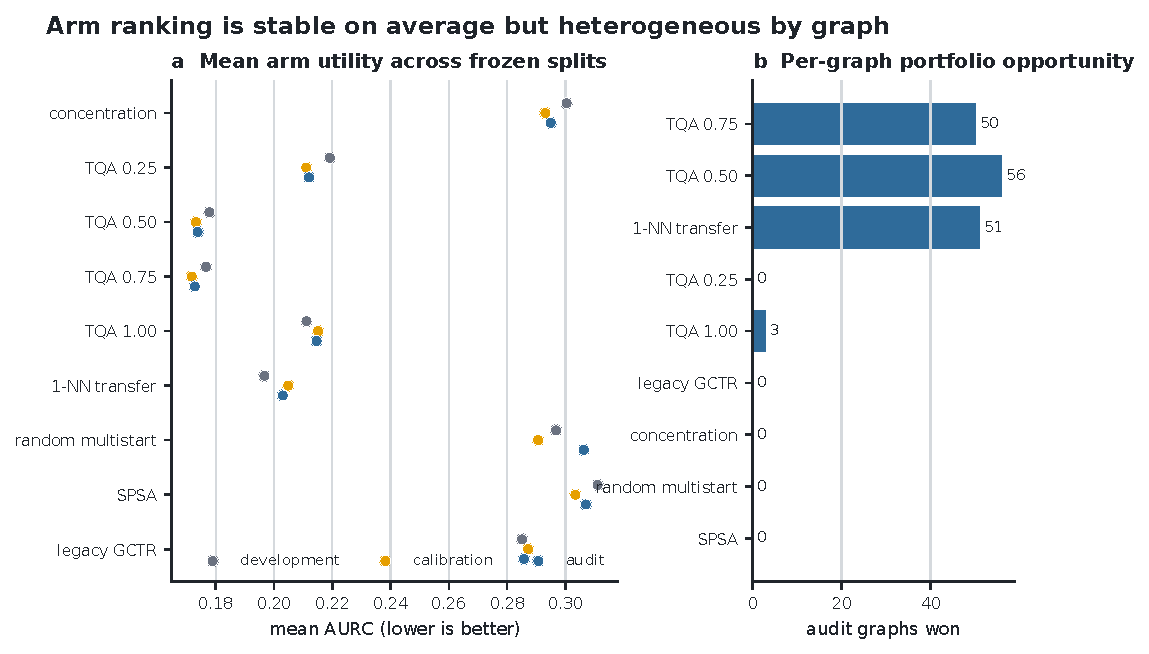
\includegraphics[width=0.98\textwidth]{figures/Figure4_ArmOpportunityRanking.pdf}
\caption{\textbf{Arm opportunity and split stability.}  \textbf{(a)} Mean utility
for every arm on the frozen development, calibration, and audit splits; lower is
better.  \textbf{(b)} Number of audit graphs on which each arm is best.
Heterogeneous graph-level winners motivate a portfolio but do not by themselves
validate a learned router.}
\label{fig:arm-ranking}
\end{figure*}

\subsection{Confirmatory Audit}

Table~\ref{tab:confirmatory} gives the locked policy comparison, and
Fig.~\ref{fig:residual-order} displays the frozen residual rule and its
inferential boundary.
The one-shot audit contains $\ConfirmN$ graphs, $40$ per family.  Gated
deployment has mean utility $\ConfirmGatedAURC$ against $\ConfirmFamilyAURC$ for
the family fallback and $\ConfirmGlobalAURC$ for the global development arm, with
per-graph oracle $\ConfirmOracleAURC$; the selected-minus-family difference is
$\ConfirmDelta$, and a frozen $4{,}000$-resample stratified percentile bootstrap
interval is $[\ConfirmCILow,\ConfirmCIHigh]$.  That interval is not the decision.
The policy accepts $\ConfirmAccepted$ routes, incurs $\ConfirmHarms$ joint harms,
and has empirical residual coverage $\ConfirmCoverage$ against nominal
$\ConfirmNominal$; since coverage is below the internally frozen threshold, the
reliability gate fails.  A binomial sensitivity model gives probability $0.249$
of observing at most $141$ covered cases under independent $0.90$ coverage, so
the miss is compatible with nominal variation yet still fails the literal frozen
rule.  Family-conditional gains are heterogeneous: the improvement is largest for
random regular graphs ($\ConfirmRRdelta$) while Barab\'asi--Albert graphs
regress ($\ConfirmBAdelta$) and Watts--Strogatz graphs move slightly
($\ConfirmWSdelta$).

\begin{table*}[tbp]
\centering
\caption{\textbf{Confirmatory results and policy comparison.}
\textbf{(a)} Family-stratified audit results, where lower utility is better and
$\Delta$ is gated minus family fallback.  \textbf{(b)} Locked policies on the
same 160 audit graphs; the oracle is retrospective and unavailable at
deployment.}
\label{tab:confirmatory}
\resizebox{\textwidth}{!}{\begin{minipage}{\textwidth}
\textbf{(a) Family-stratified confirmatory audit.}\par\smallskip
\begin{tabular}{@{}lrrrrrr@{}}
\toprule
Stratum & $N$ & Fallback & Gated & $\Delta$ & Accepted & Harms \\
\midrule
Erd\H{o}s--R\'enyi & 40 & 0.16439 & 0.16439 & +0.00000 & 0 & 0 \\
random regular & 40 & 0.17223 & 0.15896 & -0.01327 & 5 & 0 \\
Barab\'asi--Albert & 40 & 0.18775 & 0.19151 & +0.00376 & 6 & 4 \\
Watts--Strogatz & 40 & 0.16391 & 0.16234 & -0.00157 & 1 & 0 \\
\midrule
All & 160 & 0.17207 & 0.16930 & -0.00277 & 12 & 4 \\
\bottomrule
\end{tabular}
\par\medskip
\textbf{(b) Locked policy comparison.}\par\smallskip
\begin{tabular}{@{}lrrl@{}}
\toprule
Policy & Mean AURC & $\Delta$ versus family & Interpretation \\
\midrule
Global development arm & 0.17277 & +0.00070 & deployable control \\
Family fallback & 0.17207 & +0.00000 & deployable control \\
Gated selector & 0.16930 & -0.00277 & 12 accepted routes \\
Per-graph portfolio oracle & 0.16048 & -0.01159 & retrospective only \\
\bottomrule
\end{tabular}
\end{minipage}
}
\end{table*}

\begin{figure*}[tbp]
\centering
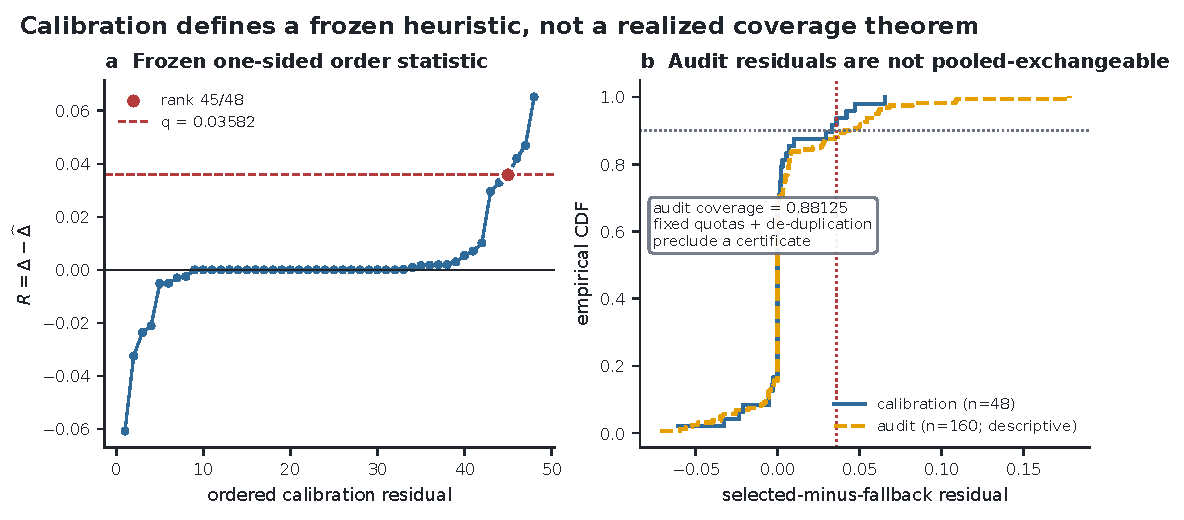
\includegraphics[width=0.98\textwidth]{figures/Figure5_ResidualOrderStatistic.pdf}
\caption{\textbf{Frozen residual rule and its inferential boundary.}
\textbf{(a)} The one-sided calibration statistic is the rank-$45$ order statistic
among $48$ residuals.  \textbf{(b)} Calibration and audit empirical CDFs are
shown descriptively.  Fixed family quotas and sequential de-duplication do not
justify a pooled exchangeability certificate.}
\label{fig:residual-order}
\end{figure*}

\subsection{Anytime Behavior and Resource Accounting}

Figures~\ref{fig:predicted-realized}, \ref{fig:anytime-family}, and
\ref{fig:family-effects} separate selective routing error, checkpoint behavior,
and family-conditional effects.
Every arm receives $32$ exact objective calls, so the audit consumes $288$ calls
per graph across nine arms and $46{,}080$ calls for the $\ConfirmN$ audit graphs;
the angle-label track is reported separately, and runtime is descriptive because
Python and simulator overhead differ by arm.  The simulator uses PyTorch for
numerical kernels \citep{paszke2019pytorch} and includes no shot noise, gate
noise, compilation, or queue latency.  Analytic gradients and higher derivatives
can be estimated on hardware under appropriate gates \citep{mari2021estimating},
and quantum-natural-gradient methods alter the local metric
\citep{stokes2020quantum}; neither is evaluated here.  The audit's statistical
unit is the graph, and the bootstrap resamples within the eight family-by-size
strata \citep{efron1993bootstrap}, so the fixed quota improves balance while
leaving the pooled sample non-iid.

\begin{figure*}[tbp]
\centering
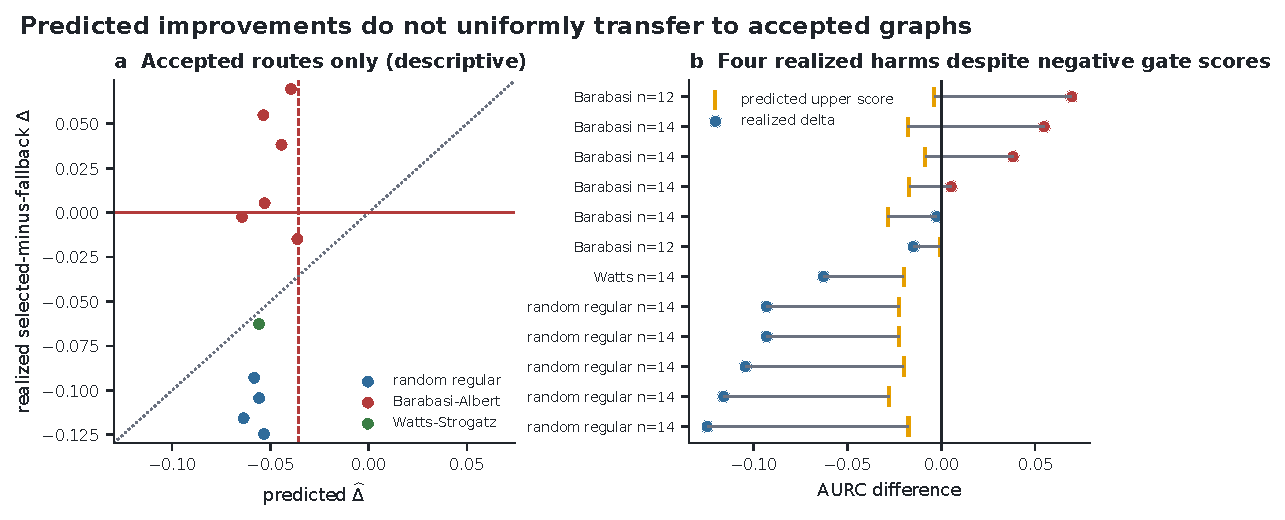
\includegraphics[width=0.98\textwidth]{figures/Figure6_PredictedVsRealizedRoutes.pdf}
\caption{\textbf{Predicted versus realized accepted routes.}  \textbf{(a)}
Predicted and realized selected-minus-fallback differences for the
$\ConfirmAccepted$ accepted graphs.  \textbf{(b)} Four accepted routes are
harmful despite negative frozen upper scores.  The display diagnoses selective
failure; it does not refit the gate.}
\label{fig:predicted-realized}
\end{figure*}

\begin{figure*}[tbp]
\centering
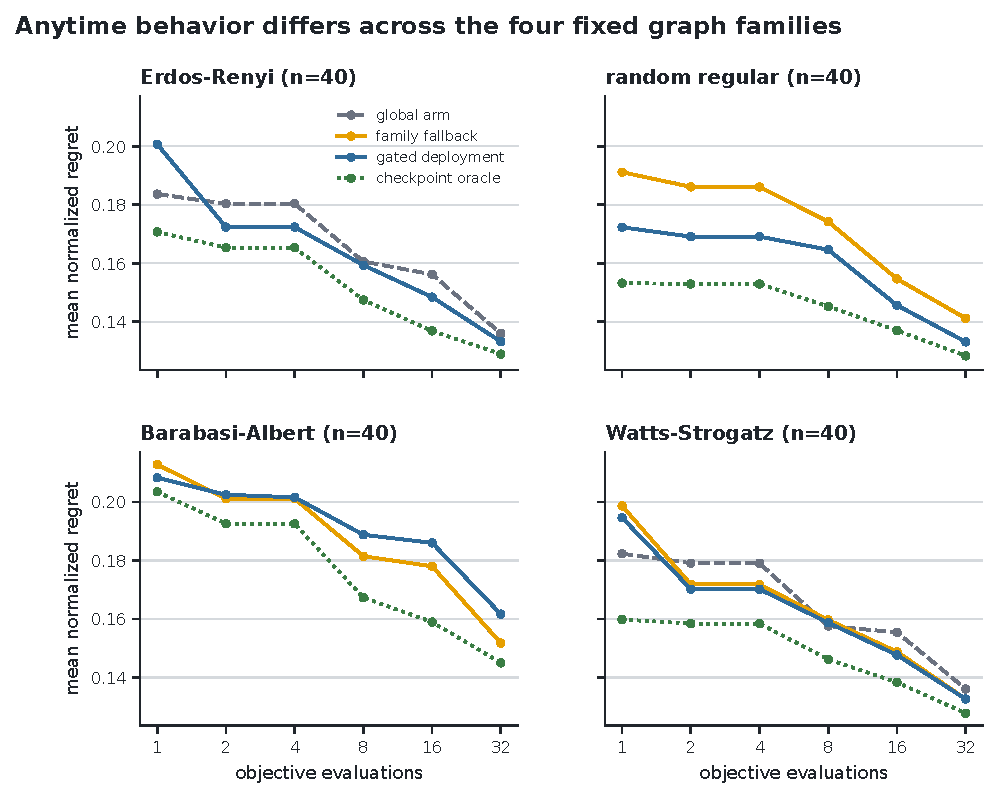
\includegraphics[width=0.98\textwidth]{figures/Figure7_AnytimeByFamily.pdf}
\caption{\textbf{Anytime behavior by fixed graph family.}  Mean normalized regret
is shown at every recorded checkpoint for the global arm, family fallback, gated
deployment, and per-checkpoint oracle.  Family heterogeneity persists across the
$32$-call budget.}
\label{fig:anytime-family}
\end{figure*}

\begin{figure*}[tbp]
\centering
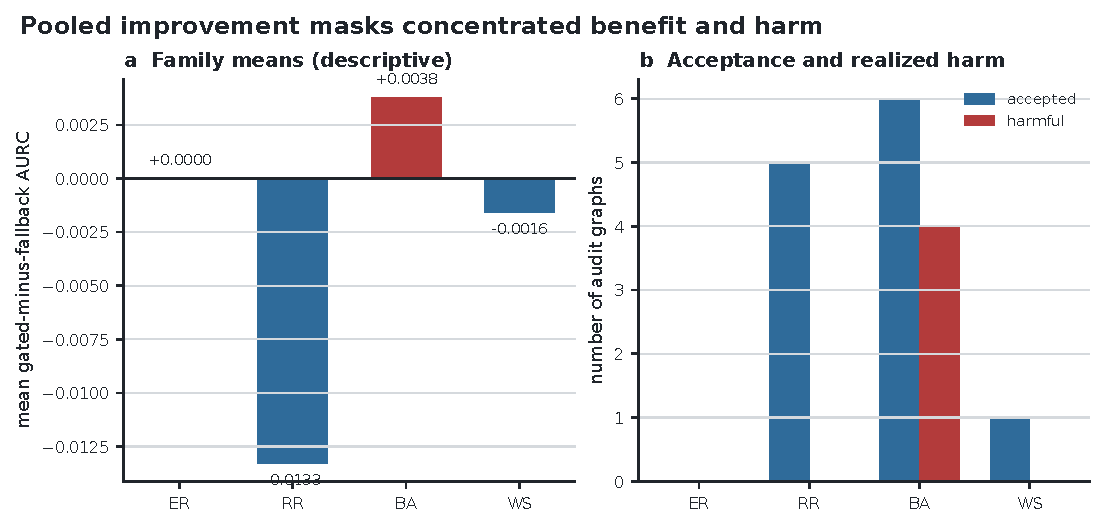
\includegraphics[width=0.98\textwidth]{figures/Figure8_FamilyEffects.pdf}
\caption{\textbf{Family-conditional effects.}  \textbf{(a)} Mean
gated-minus-fallback utility within each fixed family.  \textbf{(b)} Acceptance
and realized-harm counts.  The pooled improvement is concentrated in random
regular graphs, whereas all four observed harms occur in the Barab\'asi--Albert
stratum.}
\label{fig:family-effects}
\end{figure*}

\section{Conclusion}

Graph structure carries useful information about QAOA optimizer behavior, but
useful information is not the same as reliable routing.  The frozen selector
slightly improves mean anytime regret over a strong family fallback, yet its
accepted set is small, one third of accepted routes are harmful, and the
internally frozen empirical-coverage requirement fails, so we reject the
confirmatory reliability claim.  The value of the study is methodological:
target-free anytime utility, matched controls, split-and-lock chronology, and a
report that keeps coverage, acceptance, joint harm, and conditional harm
distinct.

\section*{Limitations}
The experiment uses exact statevectors, depth two, small unweighted MaxCut
graphs, fixed graph-family quotas, a known family label at deployment, and a
hand-designed nine-arm portfolio, and it provides no hardware, noise, asymptotic
scaling, or quantum-advantage result.  The percentile bootstrap endpoint is
boundary sensitive, and the pooled exchangeability condition required by the
simplest order-statistic theorem is not established.  A future experiment should
replace the descriptive gate with a prospective sampling design, predefine the
graph population and filtering procedure, increase accepted-route power, add shot
and device noise, and compare against stronger adaptive controls; if several
reliability criteria are tested, their multiplicity correction and joint decision
rule should be fixed before analysis \citep{benjamini1995controlling}, and any
exact binomial or concentration bound must state its independence or
exchangeability assumptions \citep{clopper1934fiducial,hoeffding1963probability}.

\section*{Data Availability}
All graph instances, locked portfolio traces, split summaries, and
machine-readable decision records used by the manuscript are included in the
public repository at
\url{https://github.com/thmolena/QAOA-Graph-Conditioned-Trust-Regions}.
The artifact manifest binds every displayed numerical file to a
SHA-256 digest and records the frozen protocol, implementation, configuration,
and decision identities.  No external or restricted dataset is required, and
no hardware data were collected.

\section*{Code Availability}
The repository contains the complete study implementation, frozen
configurations, deterministic artifact generator, validators, tests, and
source-archive builder.  Installing the repository with
\texttt{pip install .} exposes \texttt{gctr-optimize},
\texttt{gctr-portfolio}, and \texttt{gctr-reproduce-all}.  The wheel contains
its evidence bundle and supports immutable replay without the original
checkout.  Exact-statevector
calls are reported as such and are not represented as hardware shots.

\clearpage
\bibliographystyle{apsrev4-2}
\bibliography{refs}

\clearpage
\appendix

\section{Proofs}

\subsection{Proof of Theorem~\ref{thm:shift}}
\label{app:proof-shift}

\begin{proof}
Let the instance space contain two points $x_0$ and $x_1$, and define losses
\[
\begin{aligned}
 \ell(a,x_0)&=0, & \ell(b,x_0)&=\varepsilon,\\
 \ell(a,x_1)&=1, & \ell(b,x_1)&=\varepsilon,
\end{aligned}
\]
each of which lies in $[0,1]$ because $\varepsilon\in(0,1)$.  Let $P_0$ place
probability one on $x_0$ and $P_1$ probability one on $x_1$.  Under $P_0$,
$\E_{P_0}\ell(a,X)=0<\varepsilon=\E_{P_0}\ell(b,X)$, so $a$ is the unique
development risk minimizer; under $P_1$,
$\E_{P_1}\ell(b,X)=\varepsilon<1=\E_{P_1}\ell(a,X)$, so $b$ is the unique
deployment risk minimizer.  A router that unconditionally deploys the development
minimizer $a$ has deployment excess risk
\[
 \E_{P_1}\ell(a,X)-\min_{c\in\{a,b\}}\E_{P_1}\ell(c,X)
 =1-\varepsilon .
\]
Because $\varepsilon$ can be taken arbitrarily close to zero, this excess
approaches the largest possible gap for losses in $[0,1]$, and no estimation
error or model misspecification is needed to produce it.
\end{proof}

\subsection{Proof of Proposition~\ref{prop:harm}}
\label{app:proof-harm}

\begin{proof}
By the definition of conditional probability, when $\Pp(A)>0$ we have
$\Pp(H\mid A)=\Pp(A\cap H)/\Pp(A)$, and multiplying both sides by $\Pp(A)$ gives
Eq.~\eqref{eq:harm}.  For the second claim, fix any joint-harm ceiling
$\eta\in(0,1)$ and any $c\in[\eta,1]$, and construct events with $\Pp(A)=\eta/c$
and $\Pp(H\mid A)=c$; then $\Pp(A\cap H)=\Pp(A)\Pp(H\mid A)=\eta$ while the
conditional harm equals $c$.  Taking $c=1$ and $\Pp(A)=\eta$ in particular yields
joint harm $\eta$ with every accepted route harmful.  Thus a bound on
$\Pp(A\cap H)$ alone cannot imply any nontrivial bound on $\Pp(H\mid A)$ unless
acceptance is bounded away from zero, which is the assertion of the proposition.
\end{proof}

\subsection{Proof of Proposition~\ref{prop:containment}}
\label{app:proof-containment}

\begin{proof}
Take any outcome in $A\cap H$.  Membership in $A$ gives $\widehat d+q<0$, hence
$-\widehat d>q$, and membership in $H$ gives $\Delta>0$.  Therefore
\[
 R=\Delta-\widehat d>-\widehat d>q ,
\]
so the outcome lies in $\{R>q\}$; since the outcome was arbitrary,
$A\cap H\subseteq\{R>q\}$, which is Eq.~\eqref{eq:containment}.  Taking
probabilities of both sides of the inclusion gives
$\Pp(A\cap H)\le\Pp(R>q)=1-\Pp(R\le q)$.  If $\Pp(R\le q)\ge1-\alpha$ then the
right-hand side is at most $\alpha$, so $\Pp(A\cap H)\le\alpha$; and when
$\Pp(A)>0$, dividing by $\Pp(A)$ gives $\Pp(H\mid A)\le\alpha/\Pp(A)$.  Each step
follows from the deterministic containment and the definition of conditional
probability, and no exchangeability assumption enters this argument;
exchangeability is relevant only to establishing the separate premise
$\Pp(R\le q)\ge1-\alpha$ from calibration data.
\end{proof}

\subsection{Proof of Proposition~\ref{prop:quota}}
\label{app:proof-quota}

\begin{proof}
Uniformly randomizing the audit order is equivalent to choosing the $n_f$
positions occupied by family $f$ uniformly among the $\binom{n}{n_f}$ subsets of
size $n_f$.  For any position $i$,
\[
 \Pp(Z_i=1)=\frac{\binom{n-1}{n_f-1}}{\binom{n}{n_f}}=\frac{n_f}{n}=p_f ,
\]
and for distinct positions $i\ne j$,
\[
 \Pp(Z_i=1,Z_j=1)=\frac{\binom{n-2}{n_f-2}}{\binom{n}{n_f}}
 =\frac{n_f(n_f-1)}{n(n-1)} ,
\]
with the convention $\binom{N}{k}=0$ for $k<0$, which also covers $n_f=1$.
Therefore
\begin{align*}
 \operatorname{Cov}(Z_i,Z_j)
 &=\frac{n_f(n_f-1)}{n(n-1)}-\frac{n_f^2}{n^2}\\
 &=-\frac{n_f(n-n_f)}{n^2(n-1)}
 =-\frac{p_f(1-p_f)}{n-1} ,
\end{align*}
which is strictly negative because $0<n_f<n$.  Independent Bernoulli variables
have zero covariance, so the family indicators cannot be independent; their joint
law is invariant under permutations of positions, hence exchangeable.  Finally,
iid sampling from a mixture with family probability $p_f$ would give a binomial
family count with variance $np_f(1-p_f)>0$, whereas the quota design fixes that
count at $n_f$ with variance zero, so the design is not pooled iid mixture
sampling.
\end{proof}

\subsection{Proof of Theorem~\ref{thm:order}}
\label{app:proof-order}

\begin{proof}
Because $R_1,\dots,R_{n+1}$ are exchangeable and almost surely distinct, the rank
\[
 \operatorname{rank}(R_{n+1})=1+\sum_{i=1}^{n}\mathbf 1\{R_i<R_{n+1}\}
\]
is uniform on $\{1,\dots,n+1\}$.  Let $q$ be the $k$th smallest calibration
score.  If $k=n+1$, the convention $q=+\infty$ gives
$\Pp(R_{n+1}\le q)=1=k/(n+1)$ and the claim holds, so assume $1\le k\le n$.  If
the test rank is at most $k$, then at most $k-1$ calibration scores are smaller
than $R_{n+1}$, so the $k$th calibration score is at least $R_{n+1}$ and
$R_{n+1}\le q$; if the test rank exceeds $k$, then at least $k$ calibration
scores are smaller and $R_{n+1}>q$.  Hence
$\{R_{n+1}\le q\}=\{\operatorname{rank}(R_{n+1})\le k\}$, and uniformity of the
rank gives $\Pp(R_{n+1}\le q)=k/(n+1)$.  Finally
$k=\lceil(n+1)(1-\alpha)\rceil\ge(n+1)(1-\alpha)$, so dividing by $n+1$ yields
$\Pp(R_{n+1}\le q)\ge1-\alpha$.
\end{proof}

\section{Frozen Structural Routing}
\label{app:algorithm}

\noindent\textbf{Frozen structural-routing procedure.}
Given a graph $G$, development standardization, ridge coefficients, a family
fallback map, and the order statistic $q$:
\begin{enumerate}
\item compute the $16$ relabeling-invariant summaries $x(G)$;
\item standardize them using development means and scales;
\item predict all nine utilities with Eq.~\eqref{eq:ridge};
\item choose $s=\argminop_a\widehat u_a(x)$ and retrieve $b(f)$;
\item accept $s$ only if $\widehat u_s-\widehat u_b+q<0$; otherwise deploy $b$;
\item run the deployed arm under a hard $32$-call counter and record every
best-so-far checkpoint.
\end{enumerate}
The audit implementation additionally verifies that the graph, configuration,
decision, and implementation hashes match the frozen manifest before any
evaluation.  The nine arms combine model-based and model-free search;
Gaussian-process optimization is a natural future arm
\citep{snoek2012practical,balandat2020botorch}, and randomized low-rank models
may reduce structural fitting cost on much larger feature sets
\citep{martinsson2020randomized}, though neither is needed for the released
$16$-feature ridge fit.

\section{Risk Quantities and Reliability Sensitivity}
\label{app:risk}

Ridge predictions carry estimation error from finite development data, model bias
from linearity, and distribution shift across strata, while the
selected-minus-fallback residual additionally contains selection-induced
dependence because the selected arm is an $\argminop$ of the same prediction
vector; calibration treats the resulting scalar as a conformity score without
assuming Gaussianity.  Figure~\ref{fig:risk-sensitivity} pairs empirical
coverage-failure, joint-harm, and conditional-harm rates with one-sided
exact-binomial upper bounds under a hypothetical iid model: the $141$ covered
residuals out of $\ConfirmN$ fall below the literal $0.90$ requirement, and a
binomial model with success probability $0.90$ places lower-tail probability
$0.249$ on that count.  These are sensitivity analyses, not certificates for the
dependent fixed-quota design.  Broader operator portfolios could eventually
motivate shadow-tomography or classical-shadow measurement
\citep{aaronson2018shadow,huang2020shadows}, but the present commuting MaxCut
objective does not require them.  The released legacy optimizer-ablation
artifact remains a reproducible historical development diagnostic and is kept
outside the locked confirmatory portfolio decision.

\begin{figure*}[t]
\centering
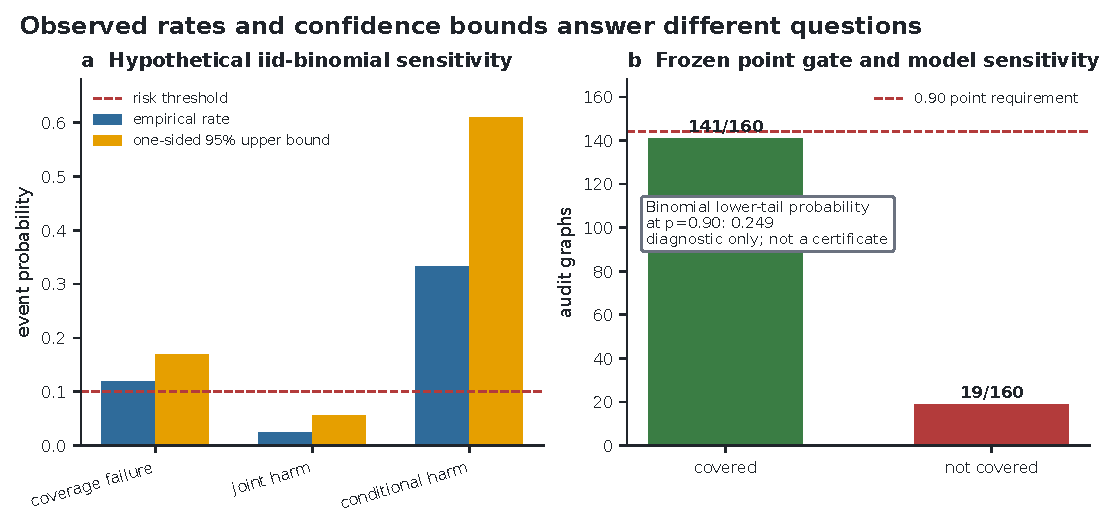
\includegraphics[width=0.98\textwidth]{figures/Figure9_RiskSensitivity.pdf}
\caption{\textbf{Risk quantities are not interchangeable.}  \textbf{(a)}
Empirical coverage-failure, joint-harm, and conditional-harm rates with one-sided
exact-binomial upper bounds under a hypothetical iid model.  \textbf{(b)} The
observed coverage count against the frozen point requirement.  These are
sensitivity analyses, not certificates for the dependent design.}
\label{fig:risk-sensitivity}
\end{figure*}

The released legacy optimizer-ablation artifact remains a reproducible
historical development diagnostic.  It informs arm design but is excluded from
the locked confirmatory decision.

\section{Optimizer Portfolio and Frozen Arms}
\label{app:portfolio}

The concentration arm uses the coordinate-wise median of the $48$ angle-label
training vectors; four linear schedules interpolate fixed midpoint ramps;
one-nearest-neighbor transfer retrieves the closest angle-label training graph in
standardized feature space; multistart divides the budget across four seeded
starts; SPSA uses a frozen gain schedule; and the legacy trust-region arm maps
graph features to a Gaussian angle policy and a local budget rule, receiving no
extra calls.  The lowest development mean-utility arm within the known generator
family is the deployable fallback, and the structural $\argminop$ replaces it
only when Eq.~\eqref{eq:gate} certifies a negative predicted upper bound.

The frozen portfolio and its realized selection-to-deployment transitions are
given in Table~\ref{tab:portfolio-arms} and
Fig.~\ref{fig:arm-transitions}.

\begin{table*}[t]
\centering
\caption{\textbf{Frozen nine-arm portfolio.}  Every arm receives the same
$32$-call ceiling; offline labels and search rules are shown explicitly.}
\label{tab:portfolio-arms}
\resizebox{\textwidth}{!}{\begin{tabular}{@{}llllr@{}}
\toprule
Arm & Initialization & Search rule & Offline labels & Calls \\
\midrule
Concentration & coordinate-wise median label & pattern search & yes & 32 \\
TQA $d_t=0.25$ & midpoint linear ramp & pattern search & no & 32 \\
TQA $d_t=0.50$ & midpoint linear ramp & pattern search & no & 32 \\
TQA $d_t=0.75$ & midpoint linear ramp & pattern search & no & 32 \\
TQA $d_t=1.00$ & midpoint linear ramp & pattern search & no & 32 \\
1-NN transfer & nearest standardized training graph & pattern search & yes & 32 \\
Random multistart & four uniform random starts & four pattern searches & no & 32 \\
SPSA & concentration angle & $a=0.18,c=0.12,\alpha=0.602,\gamma=0.101$ & yes & 32 \\
Legacy GCTR & GIN diagonal-Gaussian mean & radius-two covariance-shaped pattern search & yes & 32 \\
\bottomrule
\end{tabular}
}
\end{table*}

\begin{figure*}[t]
\centering
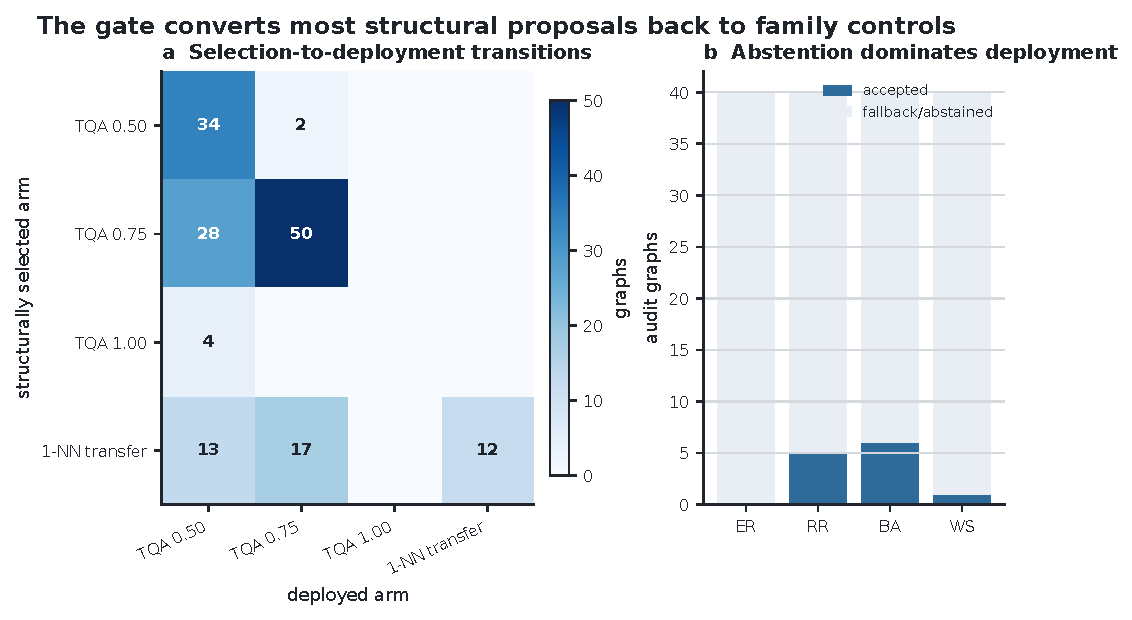
\includegraphics[width=0.98\textwidth]{figures/Figure10_ArmTransitions.pdf}
\caption{\textbf{Selection-to-deployment transitions.}  \textbf{(a)} Counts from
the structurally selected arm to the actually deployed arm.  \textbf{(b)}
Accepted and abstained graphs by family.  The gate returns most structural
proposals to their family control.}
\label{fig:arm-transitions}
\end{figure*}

\section{Split Diagnostics and Locked Gate}
\label{app:splits}

Development and calibration use disjoint graph lists, and feature
standardization, ridge fitting, family-arm means, and residual sorting use only
their assigned roles; the calibration quantile is the conservative upper order
statistic for $\alpha=0.10$.  The frozen gate applies the recorded decision rule
literally to the locked summaries and does not reinterpret a failed criterion
after audit inspection.  The confirmatory configuration fixes $20$ graphs per
family-size stratum for $\ConfirmN$ total, and the decision manifest stores the
selected arm, fallback, predicted delta, acceptance flag, and relevant hashes
before audit traces are scored.  Development-stage figures record
$\DevAccepted$ accepted routes, $\DevHarms$ joint harm, and coverage
$\DevCoverage$, with paired difference $\DevDelta$ and interval
$[\DevCILow,\DevCIHigh]$.

Table~\ref{tab:gate} records the frozen decision, and
Fig.~\ref{fig:split-diagnostics} reports the corresponding split diagnostics.

\begin{table*}[t]
\centering
\caption{\textbf{Frozen confirmatory gate.}  The empirical-coverage component
fails, so the overall decision is no-go.}
\label{tab:gate}
\resizebox{\textwidth}{!}{\begin{tabular}{@{}lrrc@{}}
\toprule
Criterion & Required & Observed & Result \\
\midrule
Portfolio opportunity & $\geq 0.05$ & 0.071 & pass \\
Global-baseline interval upper end & $<0$ & -0.000646 & pass \\
Family-fallback interval upper end & $<0$ & -0.00008178 & pass \\
Accepted audit graphs & $\geq 10$ & 12 & pass \\
One-sided empirical coverage & $\geq 0.90$ & 0.88125 & \textbf{fail} \\
Joint harm rate & $\leq 0.10$ & 0.0250 & pass \\
\bottomrule
\end{tabular}
}
\end{table*}

\begin{figure*}[t]
\centering
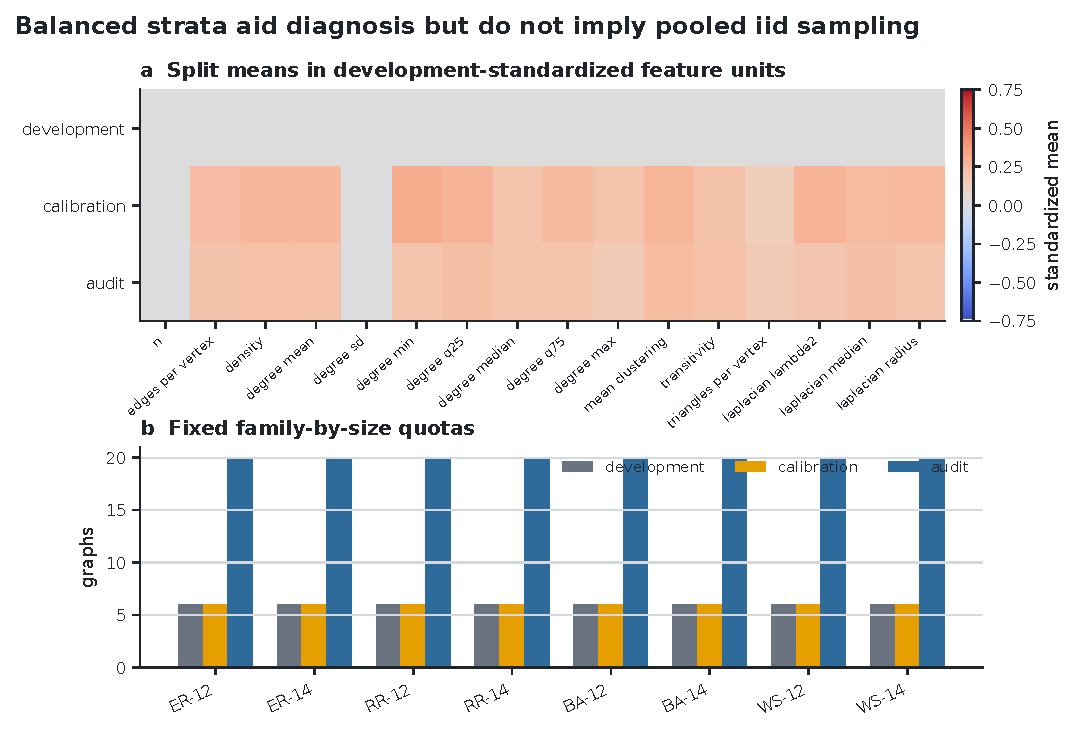
\includegraphics[width=0.98\textwidth]{figures/Figure11_SplitDiagnostics.pdf}
\caption{\textbf{Split diagnostics.}  \textbf{(a)} Feature means in
development-standardized units for development, calibration, and audit.
\textbf{(b)} Fixed family-by-size quotas.  Balance aids stratified diagnosis but
does not make the pooled sample iid.}
\label{fig:split-diagnostics}
\end{figure*}

\section{Resource Accounting}
\label{app:resource}

Every optimizer arm receives exactly $32$ objective calls: fixed schedules still
pay for their seed evaluation, multistart pays for each start from the same
counter, and model training and angle-label generation are reported outside the
deployable per-graph budget.  The displayed ledger covers the final locked
protocol and totals $79{,}488$ exact objective calls; the earlier regular-grid
and heterogeneous development-stage studies used $36{,}096$ and $51{,}840$
additional calls, so repeating all three committed evidence tracks would use
$167{,}424$ exact objective calls.  These are research-construction costs, not
the $32$-call cost of deploying one frozen arm on a new graph, and exact
statevector runtime is never converted into hardware shots.

Figure~\ref{fig:resource-ledger} and Table~\ref{tab:resource-ledger} report the
two accounting views.

\begin{figure*}[t]
\centering
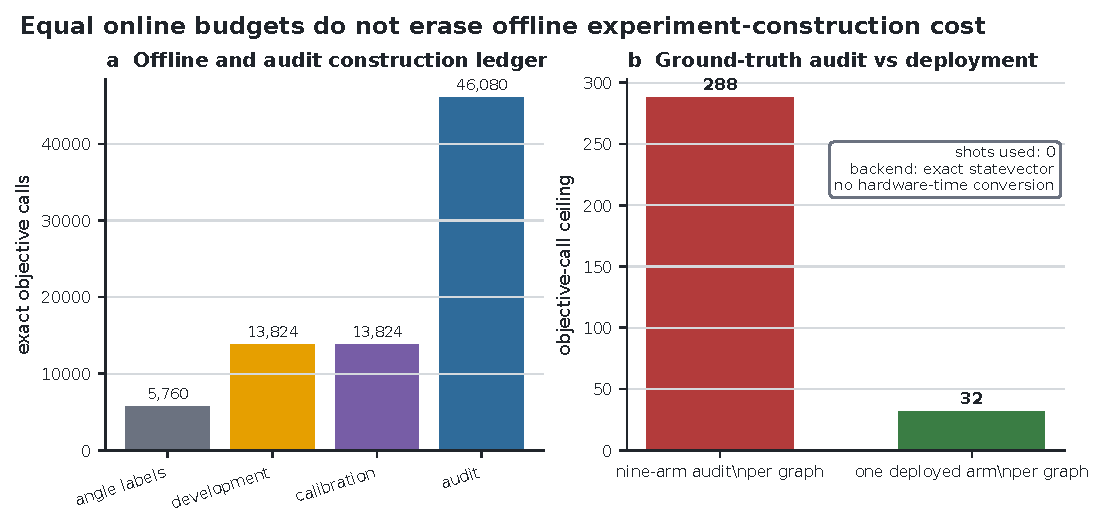
\includegraphics[width=0.98\textwidth]{figures/Figure12_ResourceLedger.pdf}
\caption{\textbf{Exact-statevector resource ledger.}  \textbf{(a)} Exact
objective calls used for angle labels, development, calibration, and the one-shot
audit.  \textbf{(b)} The nine-arm research audit is separated from the $32$-call
ceiling of one deployed arm.  No conversion to shots or hardware time is made.}
\label{fig:resource-ledger}
\end{figure*}

\begin{table*}[t]
\centering
\caption{\textbf{Final-protocol exact-statevector resource ledger.}  Query totals
are regenerated from the locked confirmatory summary; earlier development-stage
studies are reported in the surrounding text, and the deployed per-graph ceiling
is not multiplied by the nine-arm research audit.}
\label{tab:resource-ledger}
\resizebox{\textwidth}{!}{\begin{tabular}{@{}lrrl@{}}
\toprule
Stage & Graphs & Exact objective calls & Accounting role \\
\midrule
Angle-label training & 48 & 5,760 & legacy-arm labels \\
Development traces & 48 & 13,824 & nine-arm portfolio \\
Calibration traces & 48 & 13,824 & nine-arm portfolio \\
Confirmatory traces & 160 & 46,080 & nine-arm audit \\
Deployed policy & 1 & 32 & per new graph \\
\bottomrule
\end{tabular}
}
\end{table*}

The released evidence provenance record binds the protocol, implementation,
configuration, and frozen decision to complete SHA-256 values checked before
the manuscript assets are accepted.  These identities establish which
records were analyzed; they do not replace statistical validation.

The post-hoc inferential and threshold diagnostic is shown separately in
Fig.~\ref{fig:inference-threshold-sensitivity}.

\begin{figure*}[t]
\centering
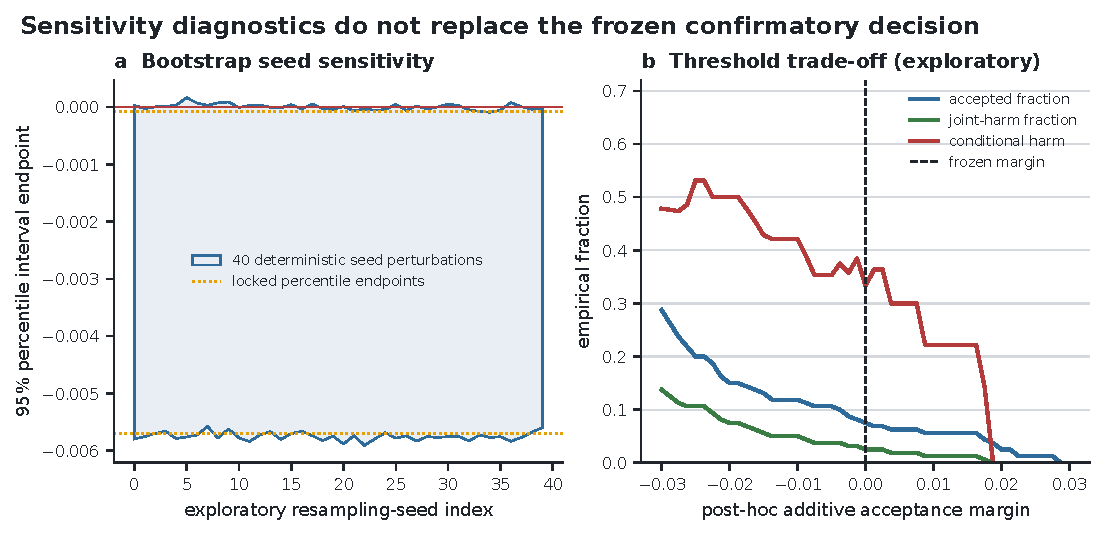
\includegraphics[width=0.98\textwidth]{figures/Figure13_InferenceThresholdSensitivity.pdf}
\caption{\textbf{Exploratory inference and threshold sensitivity.}  \textbf{(a)}
Percentile-bootstrap endpoints under deterministic resampling-seed perturbations.
\textbf{(b)} Acceptance and harm rates under post-hoc additive gate margins.
Neither panel replaces or modifies the frozen confirmatory decision.}
\label{fig:inference-threshold-sensitivity}
\end{figure*}

\end{document}
